\section{Langages de programmation}
Cette partie traite des différents éditeurs et langages de programmation utilisés dans les organisations présentées au point précédent.
\subsection{Blockly}
\label{blockly}
\begin{figure}[!h]
  \begin{center}
    
\includegraphics[scale=0.5]{content/5-related_work/images/blocky}
    \caption{Logo de Blocky}
    \label{fig:blocky}
  \end{center}
\end{figure}
Blocky\footnote{\url{https://code.google.com/p/blockly/}} est un langage de programmation graphique basé sur des technologies du web. 

Blocky est influencé\footnote{\url{https://code.google.com/p/blockly/wiki/Alternatives}} par " App Inventor " qui est influencé par "Scratch". Ce dernier est lui influencé par " StarLogo ".

Il a comme particularité :
\begin{enumerate}
\item de s'exécuter dans un navigateur ;
\item d'exporter du code source en JavaScript, Dart, etc. ;
\item d'être open source ;
\item d'être haut niveau.
\end{enumerate}

Il n'est pas directement une plate forme d'éducation dans le sens ou, suivant les blocs implémentés, il sera utilisé pour l'éducation, le business, des jeux, etc.

Lors de la conception du langage de blocky, il devait avoir certaines propriétés. Les trois premières sont pour augmenter la compréhension des néophytes, les autres portaient sur des facilités souhaitées du langage. Les propriétés décidées lors de la conception du langage sont\footnote{\url{https://code.google.com/p/blockly/wiki/Language}} :

\begin{itemize}
  \item des index de liste commençant à 1 ;
  \item des noms de variables non sensibles à la casse ;
  \item pas de portée de variable, toutes les variables sont globale ;
  \item la possibilité de faire un export en JavaScript ;
  \item un code natif généré proche de celui des blocs.
\end{itemize}

\subsection{Scratch 1}
\begin{figure}[!h]
  \begin{center}
    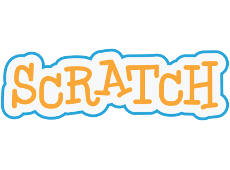
\includegraphics[scale=0.4]{content/5-related_work/images/scratch}
    \caption{Logo de Scratch}
    \label{fig:scratch}
  \end{center}
\end{figure}
Scratch est un langage de programmation développé par le MIT pour apprendre aux enfants la programmation. C'est l'interface qui permet de faire des scriptes facilement grâce à sa programmation par bloc.\\

Ce langage a été pensé pour être un outil créatif pour réaliser des histoires, des jeux, des simulations, de l'art, etc.. Ce langage a par exemple son propre éditeur d'image et de sons. Un autre but est que ce langage doit être simple à utiliser et à apprendre. Il a en effet été conçu pour des enfants n'ayant aucune connaissance préalable en programmation.\\

L'interface de Scratch se divise en plusieurs grandes parties :

\begin{enumerate}
\item sur la gauche il y a la zone de dessin dans laquelle s'anime les composants graphiques des scriptes ;
\item au milieu il y a une liste des blocs disponible trier par catégorie ;
\item sur la droite il y a la zone de scripte qui contient tous les scriptes liés au sprite sélectionné.
\end{enumerate}

\subsection{SNAP!}
\begin{figure}[!h]
  \begin{center}
    
\includegraphics[scale=0.07]{content/5-related_work/images/snap}
    \caption{Logo de SNAP!}
    \label{fig:snap}
  \end{center}
\end{figure}
SNAP est un langage de programmation de glissé déposé de blocs. C'est une ré-implémentation et une extension du langage Scratch du MIT. C'est un langage qui a été pensé et conçu pour être orienté web, ce langage est donc implémenté en JavaScript.\\

Ce langage est né en 2011 et a été créer par Jens Mönig. Il se distingue de son père Scratch par l'ajout de :
\begin{enumerate}
\item fonctions et des procédures de première classe ;
\item listes de première classe ;
\item sprite de première classe.
\end{enumerate}

\subsection{Python}
\begin{figure}[!h]
  \begin{center}
    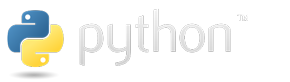
\includegraphics[scale=0.4]{content/5-related_work/images/python}
    \caption{Logo de Python}
    \label{fig:python}
  \end{center}
\end{figure}
Python est un langage de programmation qu'il ne faut plus présenté. Il a beaucoup d'avantages dont celui d'avoir une syntaxe légère et d'être facile à prendre en main. Ceci couplé à une grande communauté et beaucoup de librairies dont la fameuse \texttt{turtle} en fait un excellent langage pour démarrer dans la programmation.

Le pendant d'utiliser un vrai langage de programmation est bien sûr de devoir l'apprendre en plus d'apprendre la logique de programmation. De plus, il faut également enseigner les bonnes pratiques de codage la première fois que l'on demande à quelqu'un de programmer avec un vrai langage. 

C'est donc un choix qui ne convient pas aux trop jeunes ni à ceux qui ne sont pas vraiment investis dans l'apprentissage de la programmation.
